% -*- root: ../../main.tex -*- %

\section{Design decisions} % (fold)
\label{sec:design_decisions}

  - GDVSEPC
    - why?
  - wf engine partially in wf container

  - ruby / ruby on rails
    - for readability
    - because i know it,
    - easy to build restful APIs
    - docker library exists
    - drawback: speed, runtime

  - extra validator
    - defeats purpose of not sending data in gdvsepc but, just POC

  - for sake of simplicity:
    - no compiled language

  - activity types

  - export request synchronous
% section design_decisions (end)

\section{Execution Images} % (fold)
\label{sec:execution_images}

  \subsection{Workflow Image} % (fold)
  \label{sub:workflow_container}
    - application
      - process instance
      - process definition
      - activity instance
      - file helper
      - configuration

  % subsection workflow_container (end)

  \subsection{Activity Image} % (fold)
  \label{sub:activity_containers}
    - application
      - configuration
      - file helper

    - application wrapper
    - manual input wrapper
    - custom code wrapper
  % subsection activity_containers (end)
% section execution_images (end)

\section{System Components} % (fold)
\label{sec:components_implementation}
  \subsection{Workflow Definition Service} % (fold)
    \label{sub:workflow_definition_service}

    The workflow definition service is composed of three components: one container running a Ruby on Rails application which is configured to expose a JSON API, one container running a PostgreSQL database and a data volume container which provides persistent storage to that database.

    PostgreSQL was chosen as database solution for the definition service, because it supports both relational data, which is useful for storing the workflow, its elements and their relations, and the document-store-like JSONB format, which allows the schema-less storage of configuration information.
    - useful for queryable conf with dynamic structure
    In order to keep the stored data during container restarts or migrations across nodes, the database makes use of a data volume container which provides its working directory.

    The application container is granted access to the Docker daemon of its host node in form of a mounted volume in order to build and push images.

    As planned in \ref{}, the service has the model classes \texttt{Activity}, \texttt{ControlFlow}, \texttt{ProcessDefinition} and \texttt{Workflow}, which on the one hand act as object-relational mappers for persistence to the database, on the other hand ensure some validity constraints. Further, there exists a controller class for each of the aforementioned models, which provides \ac{CRUD} actions for the respective model. In order to have more fine-grained control over the serialization of a workflow, the \texttt{WorkflowFullSerializer} is used if a specific workflow is requested. It nests all relevant workflow elements into the workflow model before it is serialized.

    While the modeling logic is partially explicitly contained in the model and controller classes and implicitly in the underlying data schema, the export logic resides in the classes \texttt{ImageManager} and \texttt{ImageBuilder}, which are supported by the class \texttt{ProcessDefinitionImageSerializer}.

    The \texttt{ProcessDefinitionImageSerializer} provides the means to create the consolidated JSON representation of a process definition with all necessary information to be interpreted in order to execute the corresponding workflow.


    \begin{figure}[htbp]
      \centering
      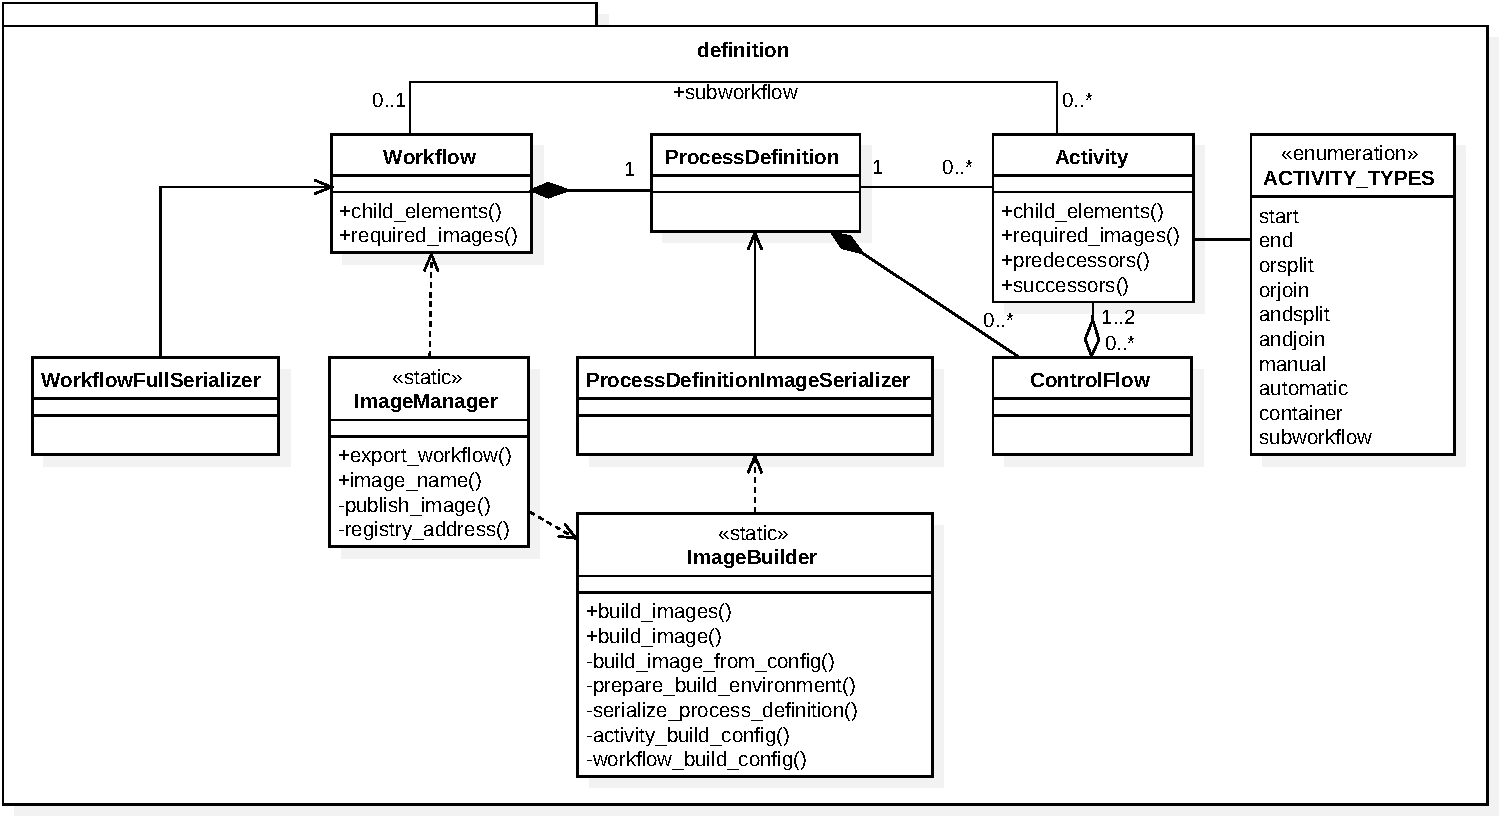
\includegraphics[width=0.95\textwidth]{content/images/class_diagram_definition-crop.pdf}
      \caption*{\scriptsize Note: Controllers omitted for the sake of simplicity. Workflow, ProcessDefinition, Activity and ControlFlow each have a controller with the respective pluralized name plus a `Controller' suffix.}
      \caption{UML Class Diagram for the Definition Service}
      \label{fig:label}
    \end{figure}


    \subsubsection{Export of a Workflow} % (fold)
      \label{ssub:exporting_a_workflow}
      If the user requests the export of a workflow, the request is forwarded to the \texttt{ImageManager}.
      In order to export a workflow, the first step is to identify all of its elements that require to be wrapped in an image. Obviously, one of them is the workflow itself. The other required images are determined by traversing the workflow's process definition recursively. Each activity has to be exported, too, and each sub-workflow has a method that exposes the Docker images it requires beyond that. It does so by passing the call for required images on to the referenced workflow, which collects its required images analogously, and returning the result.

      The \texttt{ImageBuilder} then iterates over all these elements and creates a correspondent image for each. Starting with the respective base image -- \texttt{ac\_base} or \texttt{wf\_base} -- it adds additional layers to do so. The \texttt{ImageBuilder} creates the files which are specific to the current element from the activity's or workflow's configuration, \ie the input/output validation schemata, the element's description file, and in case of a workflow the serialized process definition, in a temporary directory. The \texttt{ImageBuilder} then copies these files to the image and names it after the workflow element that it represents.

      The \texttt{ImageManager} then uploads all images that were successfully built to the private repository and publishes a notification of the successful build via the message broker.
      % subsubsection exporting_a_workflow (end)
    % subsection workflow_definition_service (end)

  \subsection{Organization Management Service} % (fold)
    \label{sub:organization_management_service}
      The organization management service is built similar to the workflow definition service. Just like it, the service consists of three Docker containers: a \ac{RoR}-based application that is backed by a PostgreSQL database with a data volume.

      As visible in Figure~\ref{fig:uml_class_diagram_organization}, the application itself is simpler than that of the workflow definition service, though. It merely consists of the classes User and Role and their respective controller classes. The RoleController offers an additional method to draw one user form all users with a certain role at random, which can be used as a rudimentary way to distribute tasks among users.

      The organization management service publishes successful CRUD events on the models to the message broker, such that the other services can react to it.

    \begin{figure}[htbp]
      \centering
      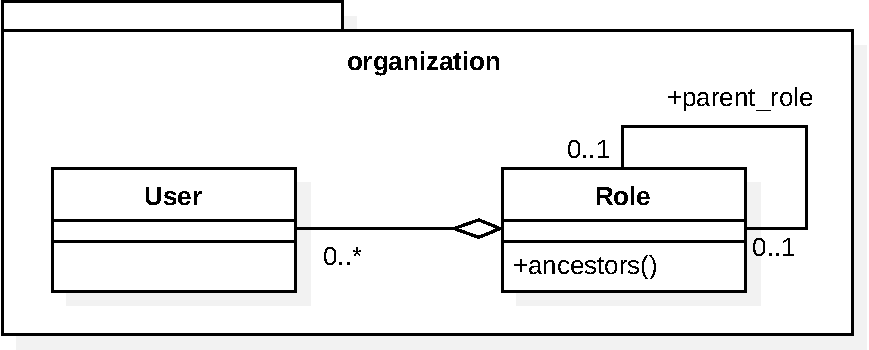
\includegraphics[width=0.65\textwidth]{content/images/class_diagram_organization-crop.pdf}
      \caption*{\scriptsize Note: Controllers omitted for the sake of simplicity. User and Role both have a controller with the respective pluralized name plus a `Controller' suffix.}
      \caption{UML Class Diagram for the Organization Service}
      \label{fig:uml_class_diagram_organization}
    \end{figure}
    % subsection organization_management_service (end)

  \subsection{Worklist Service} % (fold)
    \label{sub:worklist_service}
      The worklist service is even simpler than the organization management service. It consists of three Docker containers of the same kind, too. It only features one model class and its corresponding controller: the \texttt{WorklistItem} and the \texttt{WorklistItemController}.

      Worklist items may be queried by the identifier of the assigned user. They contain a JSON schema that describes the expected data and, after they have been worked on, the data itself.

      TODO
      % - reacts to
      %   - user created/deleted/updated
      %   - workflow finished
      %     - remove
    % subsection worklist_service (end)

  \subsection{Workflow Engine Service} % (fold)
    \label{sub:workflow_engine_service}
      - application
    % subsection workflow_engine_service (end)

  \subsection{Developer Gateway} % (fold)
    \label{sub:developer_gateway}

      Since it only offers a unified user interface for the \ac{WfMS}' services and does not store any data itself, the developer gateway does not require any database. Hence, it consists of a single Docker container that wraps a \ac{RoR} application. This application is realized in a two-tier architecture, with a backend part, which fetches data from the various services of the \ac{WfMS}, and a frontend part, which presents that data to the developer and accepts his or her input.

      - must expose ports

      \subsubsection{Backend} % (fold)
      \label{ssub:backend}
        The only task of the backend is forwarding requests to the appropriate services and their responses to the user. The model and controller classes are thus very lean. The model classes are built upon \texttt{ActiveResource}, a \ac{RoR} component that provides object-relational mapping for REST web services. The workflow definition service, the organization management service and the infrastructure service all serve a RESTful API, which enables a drop-in use of \texttt{ActiveResource} possible.

        Requests to the workflow engine are realized as messages sent to respective queues via the \ac{MOM}. An example for such a request is the instantiation of a workflow.

        Due to the Docker networking services, each service can simply be addressed by its container's name. As long as their required ports are not exposed on the host's network interface, any number of containers may be reachable on the same port. This is especially beneficial for running multiple containers that offer the same application, since they all can use their default ports this way.
      % subsubsection backend (end)

      \subsubsection{Frontend} % (fold)
        \label{ssub:frontend}
          - forms for data manipulation
          - visual workflow modeling
          - infrastructure:
            - display available nodes + ip
            - display installed images and running containers

        % subsubsection frontend (end)
    % subsection developer_gateway (end)

  \subsection{User Gateway} % (fold)
    \label{sub:user_gateway}
    Just like the developer gateway, the user gateway does not require any storage mechanism. It thus also consists of only one Docker container, which contains the \ac{RoR} application.

    - must expose ports

      - application
        - backend: rails
        - frontend: angular app
    % subsection user_gateway (end)

  \subsection{Message Oriented Middleware} % (fold)
    \label{sub:message_oriented_middleware}
      For this prototype, RabbitMQ was chosen as message oriented middleware, because it is well documented and has various ruby clients, \eg \emph{Hutch} and \emph{Bunny}.

      RabbitMQ exists as a pre-configured Docker image on the Docker Hub and can thus be utilized easily. The configuration of RabbitMQ in this image takes place when the respective container is run, which allows its configuration in the \texttt{docker-compose} configuration file.
      For the sake of simplicity, no authentication mechanism was introduced besides the simple default username/password combination.
    % subsection message_oriented_middleware (end)

  \subsection{Infrastructure Management Service} % (fold)
    \label{sub:infrastructure_management_service}
      The data that this service offers -- the state of the Docker swarm and its nodes -- should be up-to-date. It is thus gathered ad-hoc when a request arrives. This proceeding makes a database obsolete, that is why the infrastructure management service solely consists of one Docker container which contains the application.

      The \texttt{EnvironmentManager} queries the Docker daemon and processes the response. It is supported by the \texttt{DockerHelper}, which provides the means to point the local Docker client at arbitrary members of the swarm or the swarm manager.

      % It could be argued, that requests to the swarm could be made directly in the developer gateway backend. This, however, would counter the \ac{MSA} principle. In case that the Docker service alters the way it returns information, the adaption to it would require

      % -- It could be argued that the functionality could also be implemented in the developer gateway, but
      %   - separation of tasks, can be adapted independently if docker API changes

      The infrastructure management service
      - application
        - app logic
          - docker helper
          - environment manager
        - controllers
          - servers controller
        - models
          - server

    % subsection infrastructure_management_service (end)

  \subsection{Registry} % (fold)
    \label{sub:registry}
    - one docker image
    - port exposed on host
    - deployed on coordination machine
    % subsection registry (end)

  \subsection{Provisioning Service} % (fold)
    \label{sub:provisioning_service}
      - application
    % subsection provisioning_service (end)
% section components (end)


\begin{figure}[htbp]
  \centering
  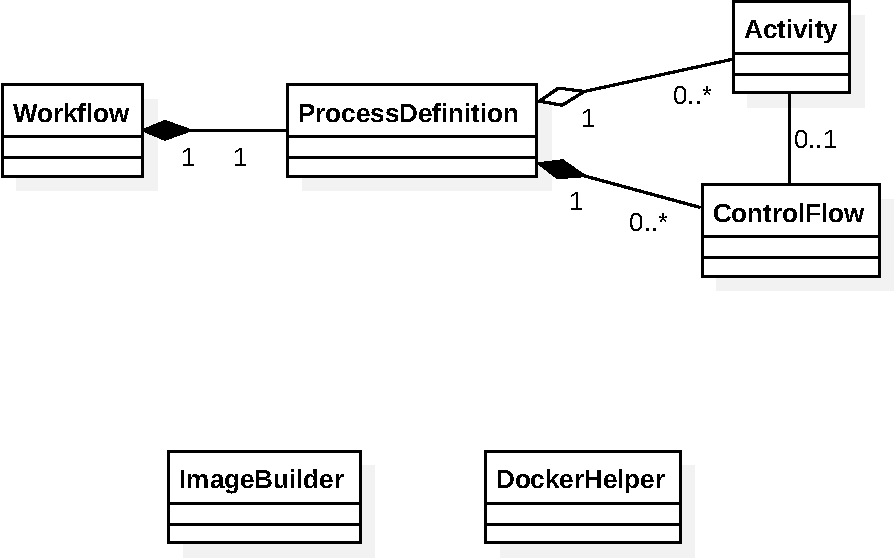
\includegraphics[width=0.95\textwidth]{content/images/class_d_definition-crop.pdf}
  \caption{UML Class Diagram of the Workflow Definition Service}
  \label{fig:uml_class_diagram_definition_service}
\end{figure}

\section{Implementation Issues} % (fold)
\label{sec:implementation_issues}

% section implementation_issues (end)
